\section{Introduction}
This is the final report presenting the term project, which aims to contribute to work on automatic summarization of long texts. This was determined to be a relevant and unsolved problem because much attention in the field of natural language processing is devoted to automatic summarization, but these algorithms focus almost exclusively on single- or multi-document short texts. However, it is a much more challenging task to summarise longer texts because approaches such as heavy reliance on the title lose their value, and the compression ratio is expected to be higher while important information is more scattered. There is nevertheless a demand for summaries of novels, and subsequently this was the specific topic chosen. Book summaries provide a quick overview to help people decide whether they want to purchase and read the book, and may also serve to refresh one's memory of a book they read previously, or as a basis for discussion of the book. Automatic summarization could be more objective and far more efficient than human summarization.

We formally define the problem as the summarization of a single-document text of over 30,000 words (with the longest in our dataset being Atlas Shrugged at over 580,000 words), to a summary of less than 1,000 words. Existing approaches can broadly be categorised into extractive and abstractive. Extractive methods directly choose important parts, usually sentences, from the original text and combine these into a summary, while abstractive methods involve rephrasing what is perceived as important. A cutting-edge approach may involve recurrent neural networks for abstractive summarization.

% summarise experiment results 

The main idea behind the work is perhaps similar to how a human may summarize long texts: by splitting the text, summarising each part and recombining, repeated until the desired length is reached. Evaluation of summaries is difficult to perform objectively and quantitatively, but BLEU and ROUGE evaluation measures have been chosen for this purpose, based on precision and recall respectively.

\section{Related Work}
%Plenty of related work has been discussed in earlier sections;~\cite{Gaikwad2016} suggests classical approaches of current automatic summarization techniques, using abstractive and extractive methods.
Most early works on 
automatic summarization focused on documentations for given text, with 
frequency of words and gauging the relatedness of each word to given or overall
context. These appearance frequencies are also used in the evaluation.

Recent researches on automatic summarization have approached in statistical
modelling and machine learning. Naturally those approaches started from the
basic techniques, and so most approaches were made with extractive
methods:~\cite{2017arXiv170804439V}. Since this methodology literally extract
human language information from given text, the output is the selected subset
of input document. Thus, it is perhaps not possible to paraphrase just like
human, but it was the mainstream of this field. However, this methodology is
highly related to the frequency of word appearance, so that it is challenging
to rank seemingly-important words shown in the input document. Moreover, it is
demanding to understand basic grammar of input language in order to select
subset and reconstruct into several sentences.

As the deep learning approaches became main strategy in many researches areas,
the importance of modelling is risen, many researchers adopt some abstractive
methods in Natural Language
Processing:~\cite{2016arXiv160206023N},~\cite{2017arXiv170404368S},~and~\cite{Rush2015}.
Before, abstractive sentence summarization has been traditionally used in
headline generation, which gives intuition that abstractive methods is capable
of not only summarizing but also paraphrasing the input documents which some
understanding of human languages. 

However, most of work on automatic summarization is primarily targeting on
the summarization of article-length input document. It is found that not many
papers are dealing with the input document of book-level length, and most of
those papers are about classification task. This gives us an idea to apply
recent techniques in automatic summarization on books.


\section{Approach}

\subsection{Simple, recursive summarization}


% You can do the same for your parts if you want to avoid merge conflicts


\section{Experiments}
\subsection{Dataset}
A dataset of ten novels and a play was collected from the internet, with at
least three summaries each. The books are mainly fictional classics, due to
their popularity on summary resources and often the expiration of their
copyright. Most of the summaries are sourced from CliffsNotes, SparkNotes and
GradeSaver. The books and summaries both vary quite vastly in length. All the
documents were saved as or converted to text files, to facilitate consistency
and ease of manipulation in Python.

\subsection{Evaluation}
Aside from simply reading the summarization outputs of the algorithm, two
quantitative measures are used to evaluate them.
The nltk.translate.bleu\_score toolkit has a function, corpus\_blue, which can
be used for BLEU evaluation. BLEU was originally used for translations, but is
now also used to evaluate summaries and is based on precision scores of
n-gram overlaps between documents and references. The corpus\_blue allows for
varying weights of 1- to 4-grams, and for multiple golden references. 

In table~\ref{table:bleu_huckfinn}, example scores of running this BLEU
evaluation can be seen. In each case, one online summary was evaluated against
the other three as golden references. For pure 1-grams, the scores are always
higher than 2-grams, and indeed they were almost zero for 3- and 4-grams.
Another remark is that while scores over 0.6 seem quite high, the CliffsNotes
score is a low outlier at only 0.295 for the 1-gram case. Finally, it must be
noted that increasing the number of references also increases the score.
Because there are more versions of what a ``correct'' summary is, there is
probably also more overlap of the remaining summary to them. Because it is not
easy to obtain more summaries, the availability of only three to four per book
must simply be kept in mind as a limitation when it comes to evaluation.

\begin{table}[H]
	\centering
	\caption{Example BLEU 1-gram and 2-gram evaluation for online summaries of the Adventures of Huckleberry Finn.}\label{table:bleu_huckfinn}
	\begin{tabular}{l l l }
		\toprule
		\textbf{}   & \textbf{1-gram} & \textbf{2-gram} \\ \midrule
		CliffsNotes & 0.295           & 0.127           \\ \midrule
		SparkNotes  & 0.646           & 0.260           \\ \midrule
		GradeSaver  & 0.655           & 0.262           \\ \midrule
		Wiki   & 0.646           & 0.234           \\
		\bottomrule
	\end{tabular}
\end{table}

Additionally, ROUGE (recall-oriented understudy for gisting evaluation) is also
used for evaluation; the score is based on recall of n-gram overlaps between
system and golden summaries. Because higher n-gram scores are so low, 1- and 2-
grams of each BLEU and ROUGE were the main metrics used. In evaluating, words
were stemmed, stop-words were accounted for and punctuation was removed, in
order to focus on content rather than phrasing.

\subsection{Results}
Because of the novelty of the method, there were no established baselines to
compare to. As ROUGE and BLEU scores would also vary wildly with the dataset
used, it would also not make sense to compare these to other studies. In terms
of purely quantitative scores, promising results were obtained, in the sense
that the system summaries scored similarly to the golden summaries against each
other.

In the experiments, the effect of changing various parameters was examined. The
first of these was the sizes of the sections that the book was broken into.
This was varied between 10 and 100 sentences, while the number of sentences out
from each chunk was kept constant at 5 sentences. In
Appendix~\ref{appendix:countfigs}, figure~\ref{fig:bleus_okay} shows an example of these
results for the Alchemist. From this, it was found that performance was roughly
constant for sentence chunks up to 50, after that it drops. This indicates that
when output sentences drop to less than 10\% of input sentences in each step,
the information retention drops.

In another experiment, the chunk size was kept constant at 50 sentences, but
the number of sentences output from these was varied between 1 and 45. From
figure~\ref{fig:bleus}, it can be seen that there is an optimum at 10 sentences
out for 50 sentences in, for the Alchemist but also observed in other books.
More interestingly, these experiments were repeated both with and without using
the important words to weight sentences. While weighting did not make any
significant difference in the BLEU-1 score, it consistently improved BLEU-2
score. This indicates that more important and informative sentences were
selected due to the weighting. Additionally, BLEU-1 scores around 0.5 and
BLEU-2 around 0.15, which are each only around 0.6 lower than golden references
evaluated against the others.

We also ran the ROUGE evaluation script for the summaries of The Alchemist. For
generating our summary we used a chunk size of 50, an output of 10, important
nouns were weighted at 1.5 and the final summary length limit was set to a 1000
words. The results are in the table~\ref{tab:rouge-alchemist}. As we can see,
our summary performs okay; In all the categories it has a higher score than the
GradeSaver summary.

\begin{figure}[H]
	\centering
	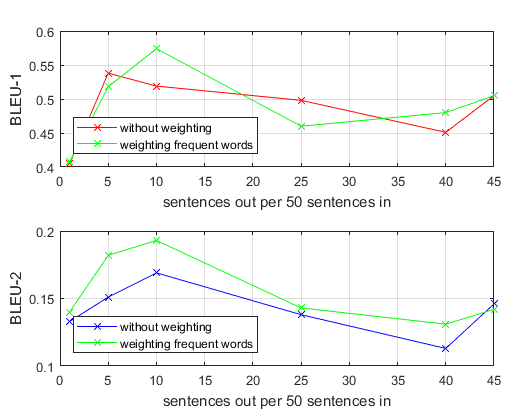
\includegraphics[width=1\linewidth]{bleus_good}
	\caption{BLEU scores for varying the compression ratio per recursive cycle for the Alchemist.}\label{fig:bleus}
\end{figure}

\begin{table}[H]
	\centering
	\caption{ROUGE results of summaries for The Alchemist}\label{tab:rouge-alchemist}
	\begin{tabular}{l l l l}
		\toprule
		\textbf{}   & \textbf{ROUGE-1} & \textbf{ROUGE-2} & \textbf{ROUGE-SU4} \\ \midrule
		CliffsNotes & 0.350           & 0.000           & 0.087 \\ \midrule
		SparkNotes  & 0.652           & 0.273           & 0.295 \\ \midrule
		GradeSaver  & 0.105           & 0.000           & 0.031 \\ \midrule
		Our summary & 0.120           & 0.042           & 0.045 \\
		\bottomrule
	\end{tabular}
\end{table}



\section{Discussion and Conclusions} % and future work


